% Presentación para el seminario de tesis (COLMEX). Compilar: latexmk -pdf presentacion.tex
% Gráficas: python figuras.py (solo lee los CSV del MC base).
\documentclass[aspectratio=169,11pt]{beamer}
\usepackage[T1]{fontenc}
\usepackage[utf8]{inputenc}
\usepackage[spanish,es-nodecimaldot]{babel}
\usepackage{amsmath,amssymb,booktabs,tikz,graphicx,array}
\usetikzlibrary{arrows.meta,positioning}

\usetheme{default}
\usecolortheme{seahorse}
\definecolor{azul}{RGB}{31,95,191}
\definecolor{rojo}{RGB}{200,60,40}
\definecolor{gris}{RGB}{90,90,90}
\setbeamercolor{frametitle}{fg=azul}
\setbeamercolor{title}{fg=azul}
\setbeamercolor{structure}{fg=azul}
\setbeamertemplate{navigation symbols}{}
\setbeamertemplate{footline}{\hfill\scriptsize\color{gris}\insertframenumber\,/\,\inserttotalframenumber\hspace{1em}\vspace{0.6em}}
\setbeamertemplate{itemize items}[circle]
\setbeamerfont{frametitle}{size=\large,series=\bfseries}
\setbeamertemplate{blocks}[rounded][shadow=false]
\setbeamercolor{block body}{bg=azul!8,fg=black}
\setbeamercolor{block title}{bg=azul!8,fg=black}

\newcommand{\idea}[1]{\vspace{-0.3em}\begin{block}{}\centering\small #1\end{block}}
\newcommand{\nota}[1]{\par\vfill{\scriptsize\color{gris}#1}}
\newcommand{\ellbar}{\bar\ell_j(a)}

\title{¿Qué tanto importan las decisiones de reparación?}
\subtitle{Un mercado de autos usados en equilibrio con reparación no observada}
\author{Rodrigo Antonio Aldrette Salas}
\institute{El Colegio de México \\ Seminario de tesis}
\date{Octubre 2026}

\begin{document}

\begin{frame}
  \titlepage
\end{frame}

% =====================================================================
\begin{frame}{Motivación}
  \begin{itemize}
    \item Para muchos hogares el auto es un activo importante: comprarlo,
          venderlo y \textbf{repararlo} determina cuánto dura y cuánto vale.
    \item Los modelos estructurales del mercado de autos usados (Gillingham et al., 2022)
          tratan la salida de un auto como accidente exógeno o chatarreo: \textbf{no hay
          reparación}.
    \item Pero la reparación se \textbf{elige}: depende de su precio, del estado del auto
          y de cuánto vale el auto en el mercado secundario.
    \item Y casi nunca se \textbf{observa}: ocurre en talleres informales, sin registro.
    \item Discusiones actuales (\emph{right to repair}, obsolescencia programada, vida útil
          y emisiones del parque) requieren saber cómo responde el mercado a los costos
          de reparar.
  \end{itemize}
  \idea{Si la reparación mueve la vida y el valor de los autos, ignorarla puede sesgar lo
  que inferimos de las preferencias y de los precios.}
\end{frame}

\begin{frame}{Pregunta y contribución}
  \textbf{Preguntas}
  \begin{enumerate}
    \item ¿Cuánto se sesga el modelo de Gillingham et al.\ si los datos vienen de un
          mercado donde los hogares reparan?
    \item ¿Se puede recuperar una decisión de reparar que el econometrista \textbf{no
          observa}?
  \end{enumerate}
  \vspace{0.3em}
  \textbf{Qué hago}
  \begin{itemize}
    \item Extiendo el equilibrio estacionario de Gillingham et al.\ con un estado de
          \textbf{desgaste} $w$ y una decisión de \textbf{reparar} $r$.
    \item La identifico con Hu \& Xin (2024): el precio de reparar es una variable
          excluida.
    \item Monte Carlo: simulo paneles con reparación y estimo (i) mi modelo sin ver $r$ y
          (ii) el de Gillingham.
  \end{itemize}
  \idea{Resultado: mi modelo recupera parámetros y reparación sin sesgo; Gillingham
  subestima la utilidad marginal del dinero en 38--57\% y los precios de usados viejos.}
\end{frame}

\begin{frame}{Ruta}
  \begin{enumerate}
    \item Modelo base: Gillingham, Iskhakov, Munk-Nielsen, Rust y Schjerning (2022)
    \item Lo que agrego: desgaste y reparación
    \item Simulación e implicaciones teóricas
    \item Estrategia empírica: identificación (Hu \& Xin, 2024), Monte Carlo y verosimilitud
    \item Resultados
    \item Conclusiones y siguientes pasos
  \end{enumerate}
\end{frame}

% =====================================================================
\section{Modelo base}

\begin{frame}{Modelo base: Gillingham et al.\ (2022), \emph{Equilibrium Trade in Automobiles}}
  Equilibrio estacionario de flujos (Rust, 1985) del mercado de autos nuevos y usados.
  \begin{columns}[T]
    \column{0.52\textwidth}
    \begin{itemize}
      \item Un periodo = un año. Masa unitaria de hogares, tipos $\tau$ con distinta
            utilidad marginal del dinero $\mu_\tau$.
      \item Auto: marca $j$ y edad $a=1,\dots,\bar a$. En $\bar a$ el auto desaparece.
      \item Elecciones de un dueño: \textbf{mantener}, \textbf{intercambiar} (comprar
            otro), \textbf{quedarse sin auto}; al deshacerse: vender o chatarrear.
      \item Accidente: $\alpha_j(a)=\operatorname{logit}^{-1}(\alpha_{0j}+\alpha_{1j}a)$
            manda el auto a $\bar a$.
    \end{itemize}
    \column{0.45\textwidth}
    \begin{itemize}
      \item Precios de nuevos $\overline P_j$ y chatarra $\underline P_j$:
            exógenos (economía pequeña y abierta).
      \item Precios de usados $P(j,a)$: \textbf{endógenos}, vacían el mercado.
      \item Fricciones: costos de compra $T_b$ y de venta $T_s$.
      \item Choques de preferencias valor extremo tipo I.
    \end{itemize}
  \end{columns}
  \idea{Los precios de usados no se observan: se calculan dentro de la estimación como
  condición de equilibrio.}
\end{frame}

\begin{frame}{Gillingham: cómo decide un hogar}
  Cada año, el dueño de un auto $x$ elige la opción $d$ con mayor $\;v^d(x)+\varepsilon^d$
  (valor que el modelo calcula + gusto aleatorio). Cada valor es lo de hoy más lo de mañana:
  \vspace{-0.3em}
  \begin{align*}
    v^{\text{mantener}}(x) &= u(x) + \beta\, \mathbb E\!\left[EV(x')\mid x\right],
      \qquad u(j,a)=u_0+u_1a\\
    v^{\text{cambiar a }h}(x) &= u(h) - \mu\big[P(h) - \text{ingreso por }x\big] - T_b
          + \beta\, \mathbb E\!\left[EV(x')\mid h\right]
  \end{align*}
  \vspace{-1em}
  \begin{block}{}
    \textbf{Si $\varepsilon$ es valor extremo tipo I, salen dos fórmulas cerradas:}
    \begin{columns}[T]
      \column{0.42\textwidth}
      \centering
      Probabilidad de elegir $d$ (logit)\\[0.3em]
      $\Pi(d\mid x)=\dfrac{e^{v^d(x)/\sigma}}{\sum_{d'} e^{v^{d'}(x)/\sigma}}$
      \column{0.55\textwidth}
      \centering
      Valor de elegir lo mejor (log-suma)\\[0.3em]
      $EV(x)=\mathbb E\big[\max_d\, v^d+\varepsilon^d\big]=\sigma\log\sum_{d} e^{v^d(x)/\sigma}$
    \end{columns}
    \smallskip
    {\small La log-suma es un ``máximo suavizado'': si una opción domina, $EV$ es casi su
    valor; si hay varias parecidas, queda un poco arriba de la mejor.}
  \end{block}
  {\small $EV$ aparece a ambos lados: es un punto fijo, $EV=\Gamma(EV;P)$. Dados los precios
  $P$, da las probabilidades de elección.}
\end{frame}

\begin{frame}{Gillingham: el equilibrio y lo que deja fuera}
  \textbf{Equilibrio estacionario} $(P,q)$: \;
  $\underbrace{q\,\Omega(P)\,Q = q}_{\text{la distribución no cambia}}$
  \quad y \quad
  $\underbrace{D(P,q)=S(P,q)}_{\text{cada mercado }(j,a)\text{ se vacía}}$
  \par\smallskip
  {\small Con los parámetros del paper reproduce el mercado danés: precios que caen
  $\approx 13\%$ al año y $\approx 34\%$ de hogares sin auto.}
  \medskip

  \textbf{Para el modelo, dos autos LB de 8 años son idénticos}
  \begin{itemize}
    \item Mismo precio $P(j,a)$ y misma probabilidad de accidente $\alpha_j(a)$.
    \item Si un dueño se queda su auto y otro vende el suyo, la única explicación es
          $\varepsilon$: un gusto que se sortea de nuevo cada año.
    \item Cuidar un auto no sirve de nada: no lo hace durar más ni valer más.
    \item El gasto en reparaciones no aparece en el presupuesto del hogar.
  \end{itemize}
  \idea{Si en los datos hay autos cuidados y descuidados, Gillingham solo puede explicar
  sus diferencias con suerte ($\varepsilon$) y con los parámetros de edad.}
\end{frame}

% =====================================================================
\section{Lo que agrego}

\begin{frame}{Lo que agrego (1): el desgaste del auto $w$}
  Cada auto tiene una probabilidad $s$ de descomponerse en el año. La escribo en log-odds
  como la curva de Gillingham más una \textbf{desviación} $w$:
  \[
    \log\frac{s}{1-s}=\ellbar + w,\qquad
    \ellbar=\alpha_{0j}+\alpha_{1j}\,a+\alpha_{2j}\,a^2
  \]
  \begin{itemize}
    \item $w=0$: el auto se descompone como el promedio de Gillingham. $w>0$: más
          desgastado.
    \item Un auto nuevo nace con $w=0$. El estado del dueño es $x=(j,a,w)$.
    \item El desgaste también molesta al usarlo:
      \[
        u_\tau(j,a,w)=u_{0\tau j}+u_{1\tau j}\,a+u_w\,w,\qquad u_w<0
      \]
    \item Mercado con información simétrica: un precio por celda, $P(j,a,w)$.
  \end{itemize}
  \idea{Ahora dos autos de la misma marca y edad pueden valer distinto, y el dueño puede
  invertir en el suyo.}
\end{frame}

\begin{frame}{Lo que agrego (2): la decisión de reparar}
  \textbf{Cómo cambia el desgaste.} Si el auto sobrevive al año:
  \[
    w' = w + \underbrace{\delta_j - \gamma_j(a)}_{\text{desgaste según la edad}}
             - \underbrace{\kappa\, r}_{\text{reparar}} + \eta,
    \qquad \eta\sim N(0,\sigma_\eta^2)
  \]
  {\small $\delta_j$: desgaste anual; $\gamma_j(a)=\alpha_{1j}+\alpha_{2j}(2a+1)$: la parte
  que ya está en la curva de Gillingham.}
  \medskip

  \textbf{Cuándo se repara.} El dueño de $h=(j,a,w)$ compara costo y beneficio:
  \[
    \Delta(h)=\underbrace{-\mu R_t(j,a)}_{\text{costo hoy}}
      +\underbrace{\beta\big(\mathbb E[EV\mid r=1]-\mathbb E[EV\mid r=0]\big)}_{\text{beneficio mañana}}
  \]
  \vspace{-0.8em}
  \[
    \Pr(r=1\mid h)=\frac{1}{1+e^{-\Delta(h)/\sigma_{rep}}}
  \]
  \begin{itemize}
    \item Beneficio: un auto menos desgastado se descompone menos, es más cómodo y se
          revende más caro.
    \item $R_t(j,a)$: precio de reparar en el mercado $t$. Solo mueve la decisión, no
          la física del auto.
  \end{itemize}
\end{frame}

\begin{frame}{Secuencia dentro de un año}
  \centering
  \begin{tikzpicture}[node distance=0.5cm and 0.3cm,
      caja/.style={draw=azul!70, rounded corners, fill=azul!6, align=center,
                   font=\footnotesize, minimum height=1.2cm, text width=2.3cm},
      flecha/.style={-{Stealth}, thick, gris}]
    \node[caja] (x) {Estado\\$x=(j,a,w)$};
    \node[caja, right=of x] (c) {Comercio\\mantener / cambiar\\/ sin auto};
    \node[caja, right=of c, fill=rojo!8, draw=rojo!70] (r) {Reparar\\$r\in\{0,1\}$\\\textbf{no se observa}};
    \node[caja, right=of r] (f) {Uso y física\\accidente con\\prob.\ $s(j,a,w)$};
    \node[caja, right=of f] (w) {Si sobrevive:\\$w'=m(w,r)+\eta$\\$a'=a+1$};
    \draw[flecha] (x) -- (c);
    \draw[flecha] (c) -- node[above, font=\scriptsize]{$h$} (r);
    \draw[flecha] (r) -- (f);
    \draw[flecha] (f) -- (w);
    \draw[flecha] (w.south) -- ++(0,-0.5) -| node[pos=0.25, below, font=\scriptsize]{siguiente año} (x.south);
    \node[above=0.1cm of c, font=\scriptsize, gris] {matriz $\Omega(P,R)$};
    \node[above=0.1cm of f, font=\scriptsize, gris] {matriz $Q$};
    \node[above=0.1cm of w, font=\scriptsize, gris] {matriz $A(P,R)$};
  \end{tikzpicture}

  \vspace{0.6em}
  \begin{itemize}
    \item Nuevo equilibrio estacionario: $\;q\,\Omega(P,R)\,Q\,A(P,R)=q,\quad D(P,q)=S(P,q)$.
    \item $A$ es una \textbf{mezcla} de las dos transiciones de $w$:
      \[
        Z(w'\mid h)=\Pr(r=1\mid h)\,F_1(w'\mid h)+\big[1-\Pr(r=1\mid h)\big]\,F_0(w'\mid h)
      \]
  \end{itemize}
  \idea{El precio $P(j,a,w)$ incluye la reparación esperada: el valor de un auto depende
  de su $w$ y de lo que su dueño hará con él.}
\end{frame}

% =====================================================================
\section{Simulación}

\begin{frame}{Simulación: una economía con los parámetros de Gillingham}
  No tengo aún datos de reparación, así que \textbf{simulo} una economía que parte de la
  que Gillingham et al.\ estimaron para Dinamarca.
  \medskip
  \begin{columns}[T]
    \column{0.52\textwidth}
    \textbf{Tomado del paper}
    \begin{itemize}\small
      \item 2 tipos de hogar (mitad y mitad): pareja pobre y soltero pobre, con
            $\mu=0.113$ y $0.094$.
      \item 2 marcas: \emph{light brown} (LB, nuevo a 142 mil DKK) y \emph{heavy
            brown} (HB, 276 mil DKK).
      \item Preferencias $u_0,u_1$, costos $T_b,T_s$ y curva de accidentes $\alpha$
            (tablas 4--10).
    \end{itemize}
    \column{0.45\textwidth}
    \textbf{Decisiones propias}
    \begin{itemize}\small
      \item $\beta=0.95$; vida máxima $\bar a=25$ años.
      \item Precio de chatarra: 2 mil DKK.
      \item Todo el bloque de desgaste y reparación (siguiente lámina).
    \end{itemize}
  \end{columns}
  \medskip
  {\small Sin reparación, esta economía da lo que reporta el paper: $\approx34\%$ de
  hogares sin auto y precios que caen $\approx13\%$ al año.}
  \idea{Así, cualquier diferencia con Gillingham viene del desgaste y la reparación.}
\end{frame}

\begin{frame}{Calibración de la reparación: tres mercados}
  \begin{columns}[T]
    \column{0.4\textwidth}
    \footnotesize
    \begin{tabular}{lr}
      \toprule
      Parámetro & Valor \\
      \midrule
      $\kappa$ (efecto de reparar) & 0.25\\
      $\sigma_\eta$ (choque al desgaste) & 0.15\\
      $u_w$ (molestia del desgaste) & $-0.2$\\
      $\sigma_{rep}$ (escala del logit) & 0.3\\
      $\delta_j$ & calibrado\\
      \bottomrule
    \end{tabular}
    \medskip

    {\footnotesize $\delta_j$ se fija para que, con 30\% de reparación, los autos se
    descompongan en promedio como en Gillingham.}
    \column{0.58\textwidth}
    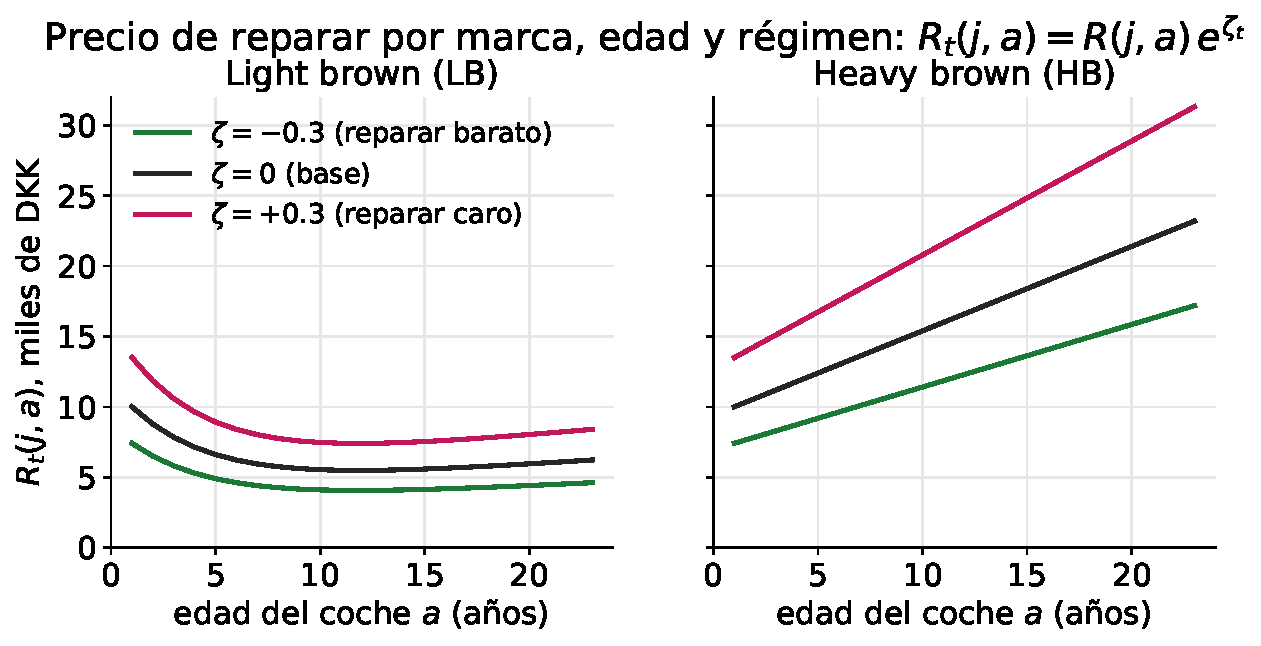
\includegraphics[width=\linewidth]{figs/fig_R.pdf}
  \end{columns}
  \medskip
  {\small Precio de reparar: LB $R=4+0.1(a-1)+6e^{-(a-1)/4}$ (caro de joven: piezas
  nuevas); HB $R=10+0.6(a-1)$. Cada mercado $t$ es igual salvo por $R_t=R\,e^{\zeta_t}$,
  con $\zeta_t\in\{-0.3,0,0.3\}$.}
  \idea{Los tres mercados son la variación que después servirá para identificar la
  reparación.}
\end{frame}

% =====================================================================
\section{Implicaciones}

\begin{frame}{Implicación 1: quién repara depende de la edad y del precio}
  \centering
  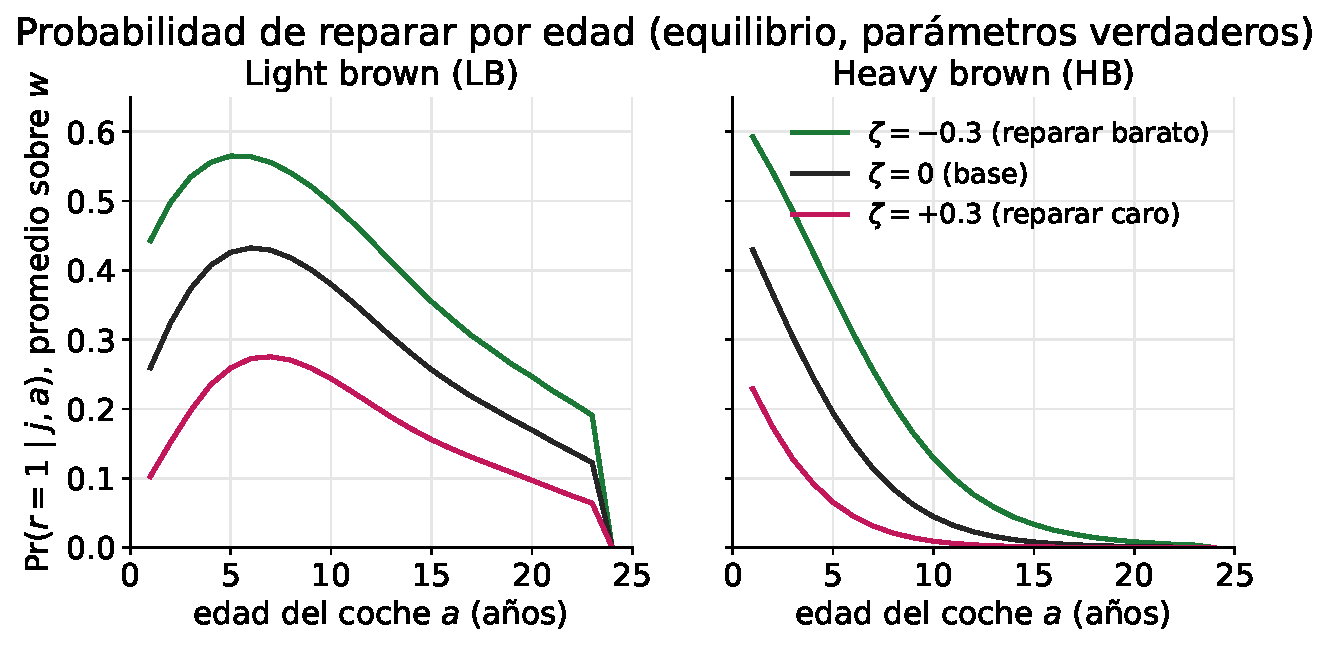
\includegraphics[width=0.72\linewidth]{figs/fig_reparar.pdf}
  \begin{itemize}\small
    \item De $\Delta(h)=-\mu R_t(j,a)+\beta\,(\text{valor de un auto menos desgastado})$:
      \begin{itemize}\small
        \item Joven: poco desgaste que frenar y $R$ alto (LB) $\Rightarrow$ poca reparación.
        \item Viejo: queda poca vida por alargar $\Rightarrow$ la ganancia cae a cero.
        \item HB: $R$ crece con la edad $\Rightarrow$ la reparación cae de forma monótona.
      \end{itemize}
    \item $\partial \Pr(r=1)/\partial R<0$: el precio de reparar mueve la curva completa.
  \end{itemize}
\end{frame}

\begin{frame}{Implicación 2: reparar barato cambia el mercado}
  Equilibrio con los parámetros verdaderos en cada mercado $t$ (promedios ponderados por $q$):
  \begin{center}\small
  \begin{tabular}{lccc}
    \toprule
    & $\zeta=-0.3$ & $\zeta=0$ & $\zeta=+0.3$\\
    & (reparar barato) & (base) & (reparar caro)\\
    \midrule
    Tasa de reparación & 0.41 & 0.29 & 0.17\\
    Desgaste medio $w$ & $-0.42$ & $-0.12$ & $0.18$\\
    Edad media del parque (años) & 10.2 & 9.8 & 9.3\\
    Hogares con auto activo & 0.64 & 0.62 & 0.60\\
    Precio LB de 10 años (miles DKK) & 62.7 & 59.0 & 54.4\\
    Precio HB de 10 años (miles DKK) & 104.0 & 99.9 & 95.6\\
    \bottomrule
  \end{tabular}
  \end{center}
  Reparar más barato $\Rightarrow$ autos menos desgastados $\Rightarrow$ duran más (parque
  más viejo) y valen más: el precio de reparar se \textbf{capitaliza} en el de los usados.
  \idea{Un modelo sin reparación atribuiría estas diferencias entre mercados a
  preferencias o a costos de transacción.}
\end{frame}

% =====================================================================
\section{Estrategia empírica}

\begin{frame}{Estrategia de identificación: Hu \& Xin (2024)}
  \textbf{Problema:} no vemos $r$. Para un auto que sobrevive, lo que vemos es la mezcla
  \[
    f_t(w'\mid h)=\big[1-p_t(h)\big]\,F_0(w'\mid h)+p_t(h)\,F_1(w'\mid h),
    \qquad p_t(h)=\Pr_t(r=1\mid h)
  \]
  \centering
  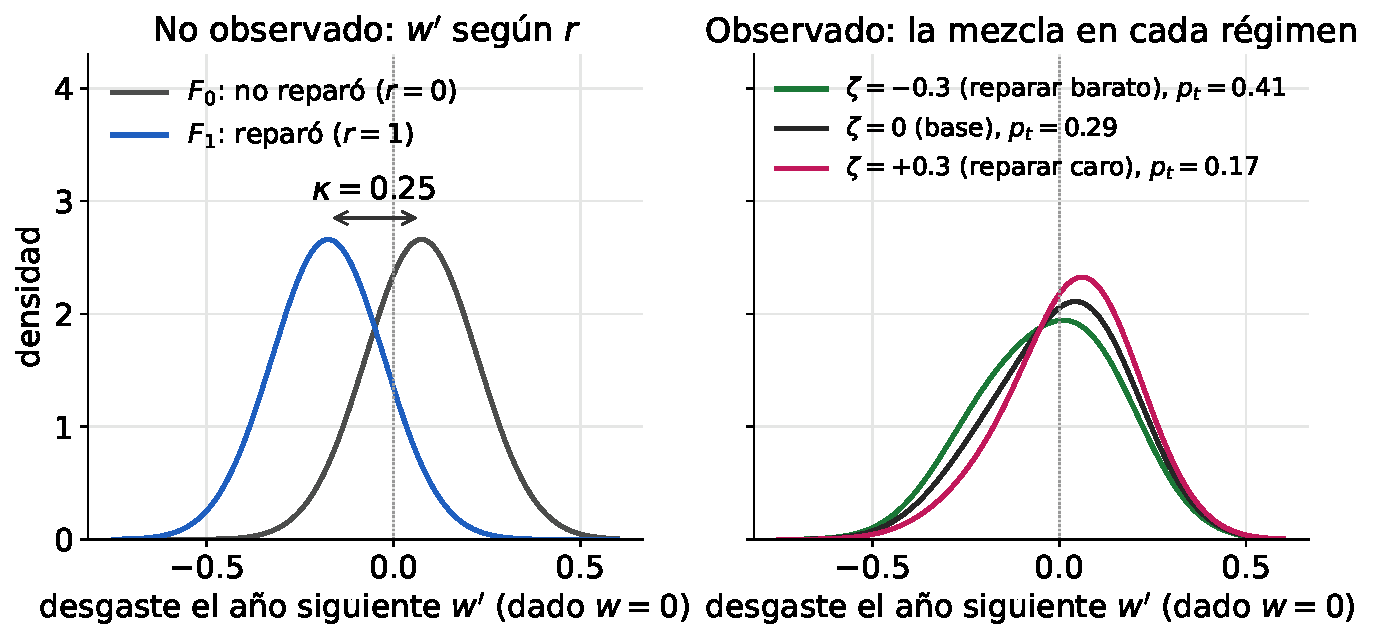
\includegraphics[width=0.7\linewidth]{figs/fig_mezcla.pdf}
  \begin{itemize}\small
    \item \textbf{Variable excluida} (Supuesto 7): $R_t$ mueve $p_t(h)$ pero no $F_0,F_1$.
          Con $\ge 2$ mercados, las mezclas distintas identifican $F_0,F_1$ y $p_t(h)$.
    \item \textbf{Choque aditivo} de media cero (Supuesto 2): por eso uso log-odds.
  \end{itemize}
\end{frame}

\begin{frame}{Monte Carlo: cómo genero los datos}
  \begin{enumerate}
    \item Con los parámetros verdaderos $\theta_0$ resuelvo el equilibrio $(P_t,q_t)$ de
          los 3 mercados.
    \item En cada mercado sorteo 10{,}000 hogares de $q_t$ y simulo sus decisiones
          durante 4 años: $\approx 90{,}000$ transiciones hogar-año.
    \item Borro lo que un investigador no vería y estimo.
    \item Repito 50 veces con paneles nuevos.
  \end{enumerate}
  \medskip
  \textbf{Qué ve el investigador} (imitando el registro danés de Gillingham):
  \begin{center}\small
  \begin{tabular}{*{3}{>{\raggedright\arraybackslash}p{0.3\textwidth}}}
    \toprule
    Siempre & Nunca & Depende del diseño\\
    \midrule
    tipo de hogar y mercado; auto $(j,a,w)$ cada año; si lo mantiene, lo cambia
    (por cuál) o se queda sin auto; $R_t$
    & precios de los usados
    & si reparó ($r$); si el auto salió por accidente o por chatarreo\\
    \bottomrule
  \end{tabular}
  \end{center}
\end{frame}

\begin{frame}{Estimación: máxima verosimilitud}
  \textbf{Idea:} elegir los $\theta$ que hacen más probable lo que observamos.
  Cada observación es un hogar que pasa de un año al siguiente:
  \[
    \hat\theta=\arg\max_\theta \sum_{\text{mercados}}\;\sum_{\text{hogares}}\;\sum_{\text{años}}
    \log \Pr\big(\text{lo observado}\mid\theta\big)
  \]
  {\small Para cada $\theta$ se resuelven los equilibrios: los precios salen del modelo.}
  \medskip

  \textbf{Ejemplo: un hogar se queda su auto y lo vemos con desgaste $w'$}
  \[
    \Pr = \underbrace{\big[1-s(h)\big]}_{\text{sobrevive}}\times
    \underbrace{Z_t(w'\mid h)}_{\text{llega a }w'}\times
    \underbrace{\Pi_t(\text{mantener}\mid w')}_{\text{decide quedárselo}}
  \]
  \textbf{Lo que no se ve se promedia con sus probabilidades}
  \begin{itemize}\small
    \item $r$ no se ve: llegar a $w'$ pondera ambos casos,
          $Z_t(w'\mid h)=p_t(h)F_1(w'\mid h)+[1-p_t(h)]F_0(w'\mid h)$.
    \item Si el auto sale del parque no sabemos si fue accidente, ni con qué $w'$
          habría seguido: se suma sobre ambos motivos y sobre todos los $w'$, cada uno con
          su probabilidad $s(h)$ y $Z_t(w'\mid h)$.
  \end{itemize}
\end{frame}

\begin{frame}{Qué se compara}
  Sobre el \textbf{mismo} panel se estiman cinco modelos:
  \begin{center}
  \begin{tabular}{llcc}
    \toprule
    & Estimador & Ve $r$ & Ve motivo de salida\\
    \midrule
    Diseño 1 & tesis, cota superior & sí & sí\\
    Diseño 2 & tesis & no & sí\\
    Diseño 3 & tesis, como datos reales & no & no\\
    Gillingham parcial & su verosimilitud (paper) & \multicolumn{2}{c}{ignora $w$ y $r$}\\
    Gillingham completa & con motivo de salida & \multicolumn{2}{c}{ignora $w$ y $r$}\\
    \bottomrule
  \end{tabular}
  \end{center}
  \textbf{Cómo se mide}
  \begin{itemize}\small
    \item \textbf{Sesgo}: cuánto se aleja el promedio de las 50 estimaciones del valor
          verdadero (en \%).
    \item \textbf{Cobertura}: en qué fracción de las 50 réplicas el intervalo de 95\%
          contiene el valor verdadero (lo ideal: cerca de 0.95).
  \end{itemize}
\end{frame}

% =====================================================================
\section{Resultados}

\begin{frame}{Resultado 1: el modelo de la tesis recupera los parámetros sin ver $r$}
  {\small Diseño 3: el caso más difícil, sin ver $r$ ni el motivo de salida.}
  \begin{center}\small
  \begin{tabular}{lrrrr}
    \toprule
    & & \multicolumn{2}{c}{Tesis (diseño 3)} & Gillingham\\
    \cmidrule(lr){3-4}\cmidrule(lr){5-5}
    Parámetro & Verdad & Sesgo & Cobertura & Sesgo\\
    \midrule
    $\mu$ (pareja) & 0.113 & $-0.5\%$ & 0.94 & $-57\%$\\
    $u_0$ (pareja, LB) & 3.65 & $-0.2\%$ & 0.94 & $-29\%$\\
    $T_b$ (pareja) & 6.59 & $+0.6\%$ & 0.90 & $+30\%$\\
    $\kappa$ (efecto de reparar) & 0.25 & $0.0\%$ & 0.94 & ---\\
    $\sigma_\eta$ (choque al desgaste) & 0.15 & $0.0\%$ & 0.96 & ---\\
    $\sigma_{rep}$ (escala del logit) & 0.30 & $-0.5\%$ & 0.96 & ---\\
    \bottomrule
  \end{tabular}
  \end{center}
  {\small En los 27 parámetros: sesgo menor a 3\% y cobertura entre 0.90 y 1.00. La tasa de
  reparación estimada es 0.276, igual a la verdadera. Los diseños 1 y 2 dan resultados
  todavía más cercanos.}
  \idea{No observar $r$ ni el motivo de salida cuesta precisión, no sesgo: la variación
  en $R_t$ basta para separar la mezcla.}
\end{frame}

\begin{frame}{Resultado 2: ignorar la reparación sesga a Gillingham}
  \begin{columns}[c]
    \column{0.62\textwidth}
    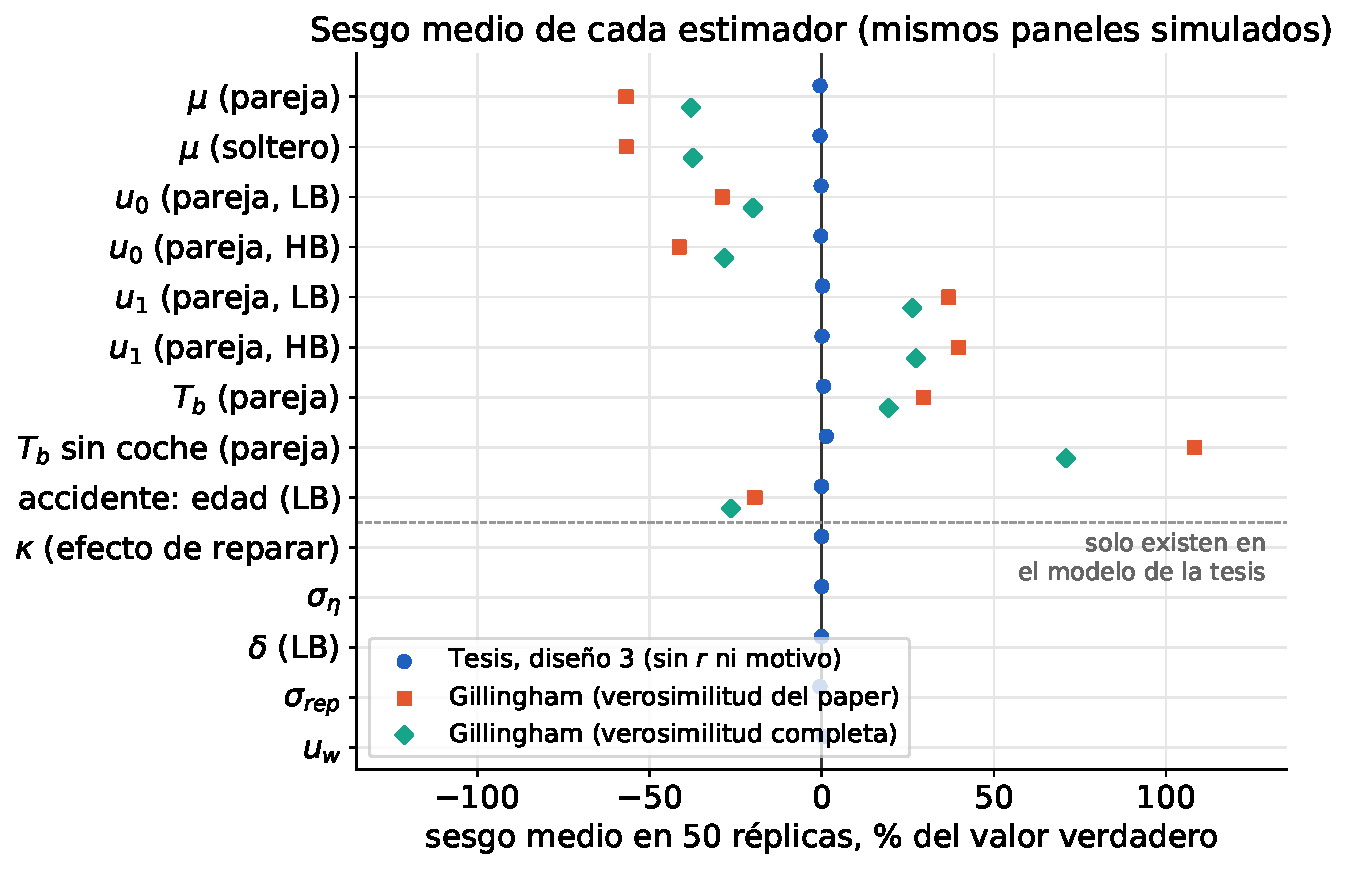
\includegraphics[width=\linewidth]{figs/fig_sesgo.pdf}
    \column{0.36\textwidth}
    \small
    \begin{itemize}
      \item $\mu$ cae 38--57\%: todo lo que se mide en dinero ($u/\mu$, $T/\mu$) sale
            inflado.
      \item $u_1$ se aplana: la pérdida de valor por desgaste se le carga a la edad.
      \item Ningún intervalo de 95\% contiene el valor verdadero.
    \end{itemize}
  \end{columns}
  \idea{Interpretación (por formalizar): sin el canal $w\to r\to w'$, Gillingham ajusta
  las mismas tenencias moviendo $\mu$, la pendiente de edad y los costos de transacción.}
\end{frame}

\begin{frame}{Resultado 3: los precios implícitos de Gillingham están sesgados}
  \centering
  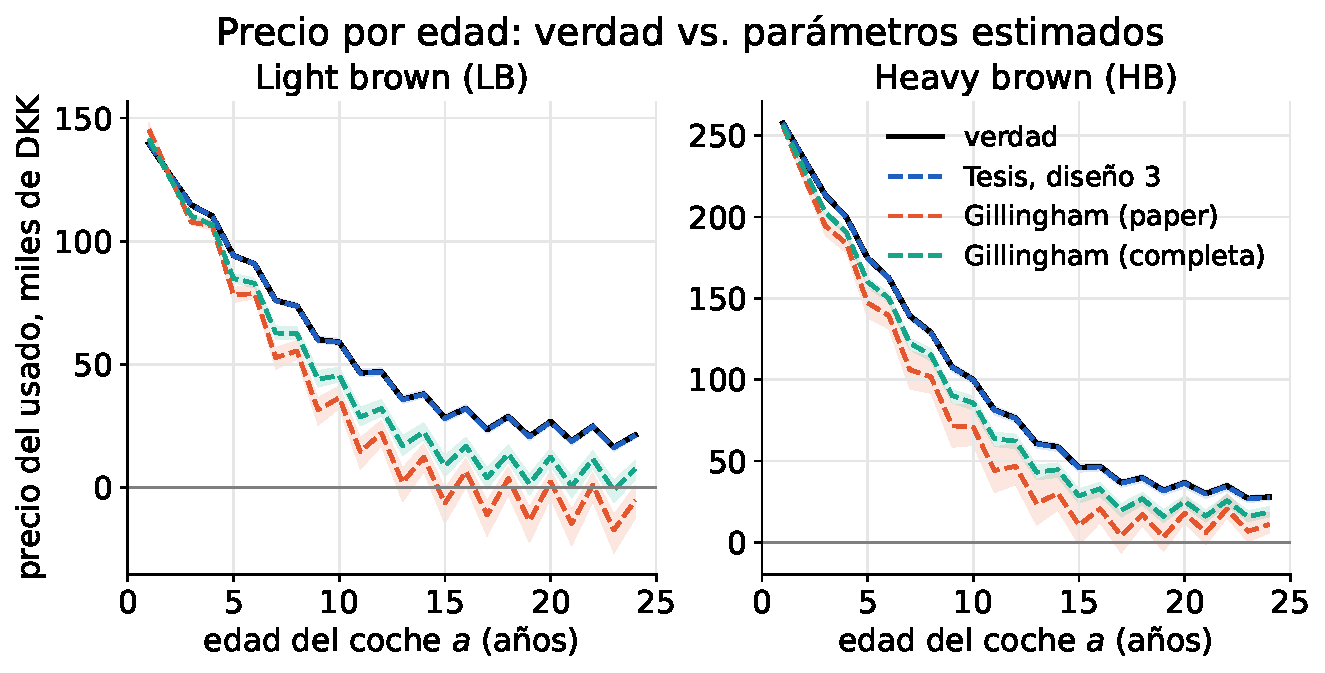
\includegraphics[width=0.68\linewidth]{figs/fig_precios.pdf}
  \begin{itemize}\small
    \item Diseño 3 (azul) cae encima de la verdad. Gillingham: $-6\%$ en edades 1--5,
          $-35\%$ en 6--12, $-94\%$ en 13--24. Precios \textbf{negativos} para LB viejos.
    \item Los precios no se observan: salen de los parámetros. Con parámetros sesgados,
          los precios de equilibrio también se sesgan.
  \end{itemize}
  \nota{Punteadas: media del equilibrio en los $\hat\theta$ de 50 réplicas; bandas: percentiles
  5--95; mercado $\zeta=0$. El zig-zag viene del costo de venta en años de inspección de la
  corrida preliminar; la final usa $T_s$ constante.}
\end{frame}

\begin{frame}{Resultado 4: \ldots aunque sí reproduce las cantidades}
  \centering
  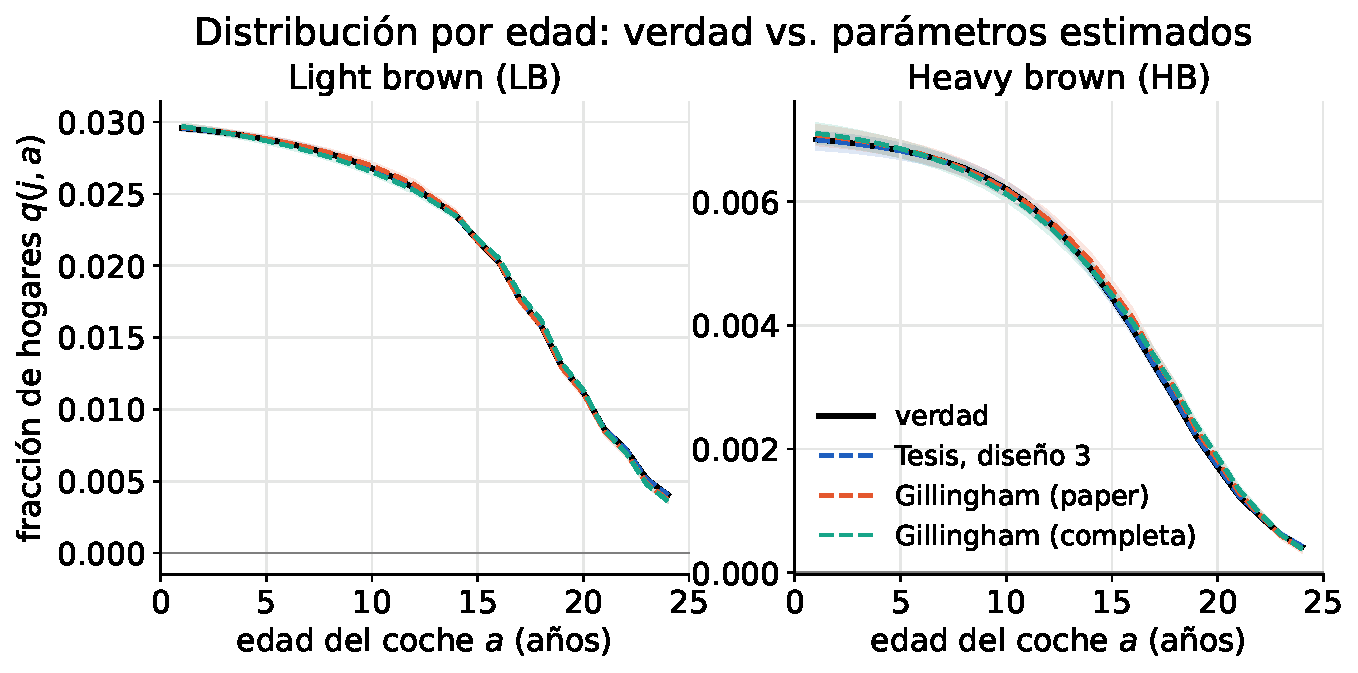
\includegraphics[width=0.68\linewidth]{figs/fig_poblacion.pdf}
  \begin{itemize}\small
    \item La distribución por edad $q(j,a)$ de Gillingham se desvía a lo más 10\%.
    \item Su verosimilitud usa tenencias y transacciones, que son justo lo que ajusta.
  \end{itemize}
  \idea{Ajustar bien las cantidades no basta para confiar en los contrafactuales: los de
  precios y bienestar dependen de $\mu$, que está sesgado.}
\end{frame}

% =====================================================================
\section{Conclusiones}

\begin{frame}{Conclusiones}
  \begin{enumerate}
    \item Agregar desgaste y reparación al equilibrio de Gillingham hace que \textbf{el
          precio de reparar se refleje en el mercado}: con reparación barata los autos
          duran más y los usados valen más.
    \item La reparación no observada \textbf{se puede identificar con variación en su
          precio} (Hu \& Xin): el modelo recupera parámetros y $\Pr(r)$ sin sesgo, aun
          sin ver $r$ ni el motivo de salida.
    \item Si el mundo tiene reparación, el modelo sin ella:
      \begin{itemize}
        \item \textbf{subestima la utilidad marginal del dinero} en 38--57\%;
        \item \textbf{subestima los precios de los usados viejos}, hasta volverlos
              negativos;
        \item y aun así \textbf{ajusta bien las cantidades}, por lo que el error no se
              nota a simple vista.
      \end{itemize}
  \end{enumerate}
  \idea{Modelar la reparación cambia lo que inferimos sobre preferencias, precios y
  bienestar en el mercado de autos usados.}
\end{frame}

\begin{frame}{Siguientes pasos}
  \begin{itemize}
    \item Corrida final del Monte Carlo con la especificación corregida ($T_s$ constante,
          edad$^2$ en la probabilidad de accidente y en la regla de desgaste).
    \item Robustez: escala del nido de $w$, $u_w=0$ (reparar solo para sobrevivir),
          tamaño de los regímenes $\zeta$.
    \item Explicar formalmente el mecanismo del sesgo en $\mu$.
    \item Contrafactuales de política: subsidio o abaratamiento de la reparación
          (\emph{right to repair}) sobre precios, vida útil y bienestar.
  \end{itemize}
\end{frame}

\begin{frame}
  \centering\Large Gracias\\[1em]
  \normalsize Rodrigo Antonio Aldrette Salas
\end{frame}

% =====================================================================
\appendix

\begin{frame}{Apéndice: árbol de decisiones de un dueño}
  \centering
  \begin{tikzpicture}[level distance=1.5cm,
      level 1/.style={sibling distance=5.2cm},
      level 2/.style={sibling distance=2.5cm},
      every node/.style={draw=azul!60, rounded corners, fill=azul!5, font=\small, align=center},
      edge from parent/.style={draw, gris, -{Stealth}}]
    \node {Dueño de $x=(j,a,w)$}
      child { node {Sin auto}
        child { node {Vender} }
        child { node {Chatarrear} } }
      child { node {Mantener}
        child { node[fill=rojo!8, draw=rojo!60] {Reparar} }
        child { node[fill=rojo!8, draw=rojo!60] {No reparar} } }
      child { node {Cambiar a $h$}
        child { node {Vender o\\chatarrear} }
        child { node[fill=rojo!8, draw=rojo!60] {Reparar o no\\el nuevo $h$} } };
  \end{tikzpicture}
  \begin{itemize}\small
    \item Rojo: no se observa. Los autos nuevos y los de edad $\bar a-1$ no se reparan.
    \item Al comprar, se elige $(j,a)$ y luego $w$ dentro de un nido de escala
          $\sigma_w=0.1$ (fija).
  \end{itemize}
\end{frame}

\begin{frame}{Apéndice: verosimilitud cuando el auto sale del parque}
  Hogar con $h=(j,a,w)$ cuyo auto desaparece y que después hace $o$ (quedarse sin auto o
  comprar $h'$). No se sabe si fue accidente ni con qué $w'$ habría seguido:
  \[
    \Pr(o\mid h) = \underbrace{s(h)\,\Pi_t(o\mid \text{terminal})}_{\text{accidente}}
      + \underbrace{\big[1-s(h)\big]\sum_{w'} Z_t(w'\mid h)\,
        \Pi_t(o,\text{chatarrear}\mid j,a+1,w')}_{\text{sobrevivió y lo chatarreó}}
  \]
  \begin{itemize}\small
    \item $Z_t(w'\mid h)=\sum_r p_t(r\mid h)F_r(w'\mid h)$ pondera cada $w'$ posible por su
          probabilidad.
    \item Como el accidente depende del $w$ de inicio de año (observado) y no de $r$, las
          dos mezclas no se cruzan: no hay selección por supervivencia.
  \end{itemize}
\end{frame}

\begin{frame}{Apéndice: construcción de $w$ y dimensiones}
  \begin{itemize}
    \item $w$ = log-odds de descomponerse menos la curva de Gillingham. Se discretiza en 71
          puntos en $[-3,2.25]$ con paso $\sigma_\eta/2$ (Tauchen), para no deformar los
          momentos con los que se separa la mezcla.
    \item En los bordes del grid $\mathbb E[\eta\mid w]\neq0$; la masa ahí es $<0.5\%$.
    \item Estados por tipo: $n=J(\bar a-1)W+J+1 = 2\cdot 24\cdot 71+3=3{,}411$.
          Precios por mercado: $3{,}408$, uno por celda $(j,a,w)$.
    \item Newton conjunto sobre $(EV_\tau,P)$ con jacobiano analítico; $\approx 130$ s por
          estimación en GPU. Errores estándar BHHH.
  \end{itemize}
\end{frame}

\end{document}
